\documentclass[border=0.2cm]{standalone}

\usepackage{tikz}
\begin{document}
\pagestyle{empty}
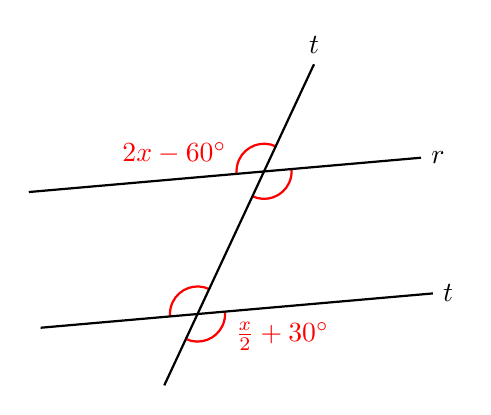
\begin{tikzpicture}[rotate=5]
    \draw (0,0) -- (240:.35cm) arc (240:360:.35cm) ;
    \draw[thick,red] (240:.35cm) arc (240:360:.35cm) node[below right] {$\frac{x}{2}+30^{\circ}$};
    \draw (-60:0.4cm);


    \draw[thick,red] (420:.35cm) arc (420:540:.35cm);
    \draw (500:0.4cm) ;
  \begin{scope}[shift={(60:2cm)}]

    \draw (0,0) -- (240:.35cm) arc (240:360:.35cm);
    \draw[thick,red] (240:.35cm) arc (240:360:.35cm) ;
    \draw (-60:0.4cm);


    \draw[thick,red] (420:.35cm) arc (420:540:.35cm) node[above left] {$2x -60^\circ$};
    \draw (500:0.4cm);
  \end{scope}

\draw[thick] (60:-1cm) -- (60:3.5cm) node[above] {$t$};
\draw[thick] (-2,1.73) -- (3,1.73) node[right] {$r$};
\draw[thick] (-2,0) -- (3,0) node[right] {$t$};

\end{tikzpicture}

\end{document}